\subsection{Conflicts}\label{ssec:conflicts}
As mentioned back in \cref{ch:uppaalmodel}, we did not enforce the physical rules of modules to the fullest. These entail that a module may not connect to another module if this module is not a neighbour and if the connection would force two modules to take up the same space. Using the transformation rules just described, we are sure that we can only generate configurations, where our modules connect to their neighbours. However the rules do not enforce that we may not make connections that result in intersection. 

With our transformation rules, the only time where intersection may happen is when a new line is created and branched out during either anti-serialization or parallelization. In the following subsubsection we describe two ways, Push Around and Push Beneath, in which we may append the stated rules to enforce the physical aspects of configurations.

\subsubsection{Push Around}
In push around we handle the case where a new off branching line intersects with an old line, by moving the new line above the old line. In the case where the new line entirely covers the old we perform the transformation depicted in \cref{fig:pusharound1}. As shown, the new line simply uses transport modules to lift itself up above the old line. These transport modules are technically not a part of the line and only serve the purpose of avoiding the intersection.

\begin{figure}[h]
\centering
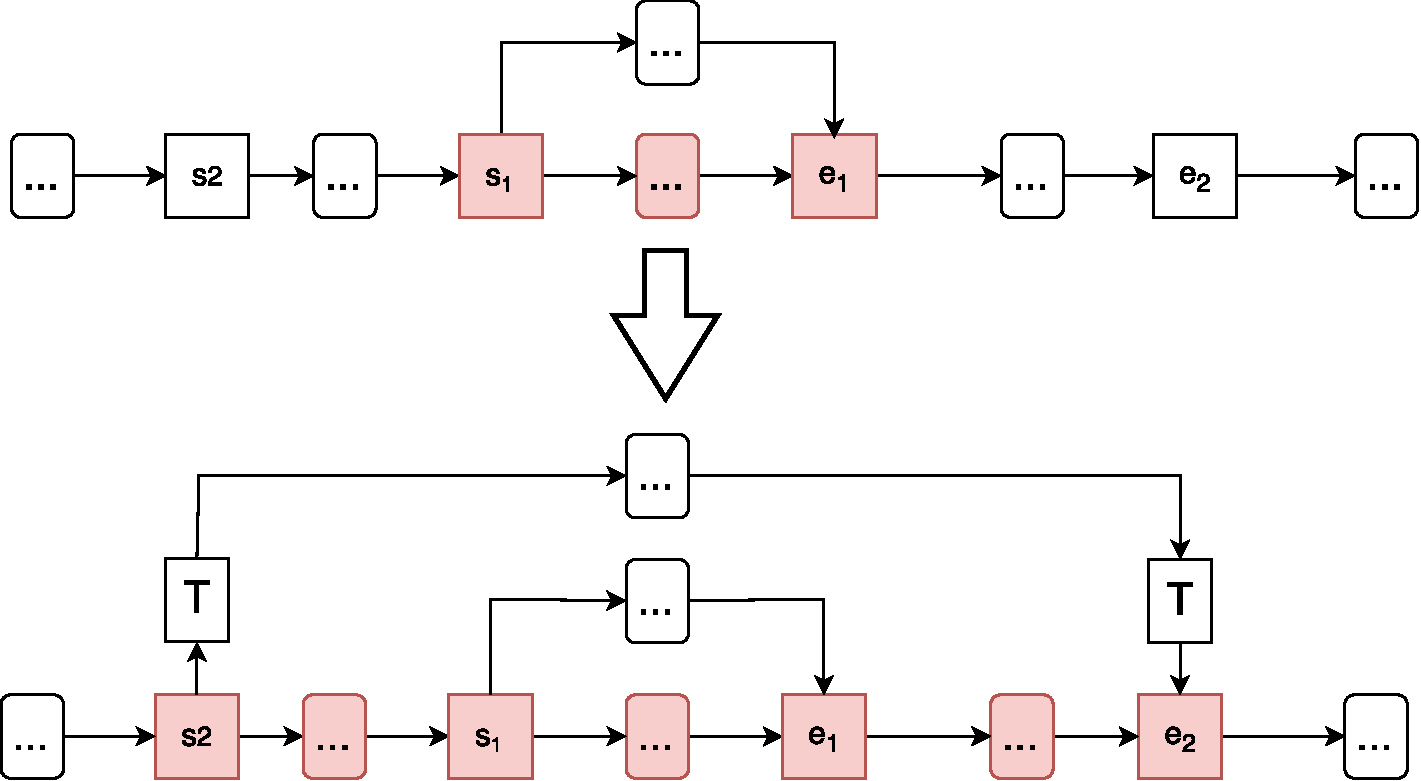
\includegraphics[width=\textwidth]{conflict1.pdf}
\caption{How push around handles the case, where we insert a new line that covers the entirety of an old line}
\label{fig:pusharound1}
\end{figure}

There is also the case where the new line is covered by the old line entirely. In this case we use the transformation in \cref{fig:pusharound2}. Here we do not need to append any transport module as we move up through the already existing modules, which we would otherwise intersect with. 

In the cases where the new entirely intersects the old it will add transport modules where needed, or otherwise guide itself vertically through modules that already exists. These examples only show the case, where a single old line is placed above the main line from which we branch off. In the case of more line levels, the new line will simply climb vertically until it finds a level where it may be placed without intersection. 

Push around is the intersect handling we use when inserting new lines as a result of anti-serialization, as there is no need to keep this new line close to the one from which it sprouted. 

\begin{figure}[h]
\centering
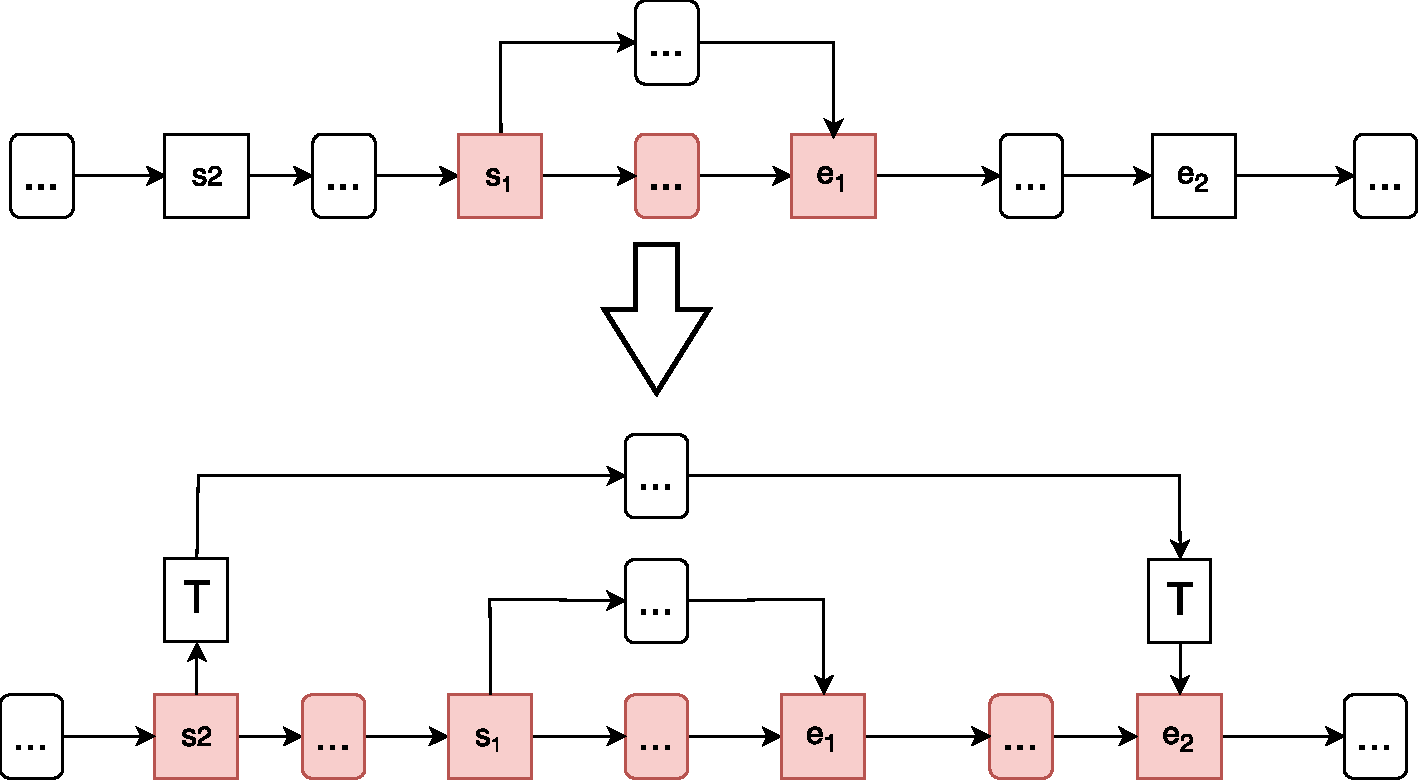
\includegraphics[width=\textwidth]{conflict2.pdf}
\caption{How push around handles the case where we insert a new line that is covered by the entirety of an old line}
\label{fig:pusharound2}
\end{figure}

\subsubsection{Push Beneath}
The other type of intersect handling that we use is called Push Beneath. Here we do the opposite of push around and handle intersection conflicts by placing the new line, where we want to place it and then moving vertically any old lines that may intersect. If this move creates another intersection we simply move the lines which we pushed into. This is done until no intersections remain. 

In the case where the new line is covered entirely by the old line we avoid intersection as in \cref{fig:pushunderneath1}. By pushing the new line up one level, we intersect the old which needs to move up as well. This warrants that the old line gets support from transport modules.

\begin{figure}[h]
\centering
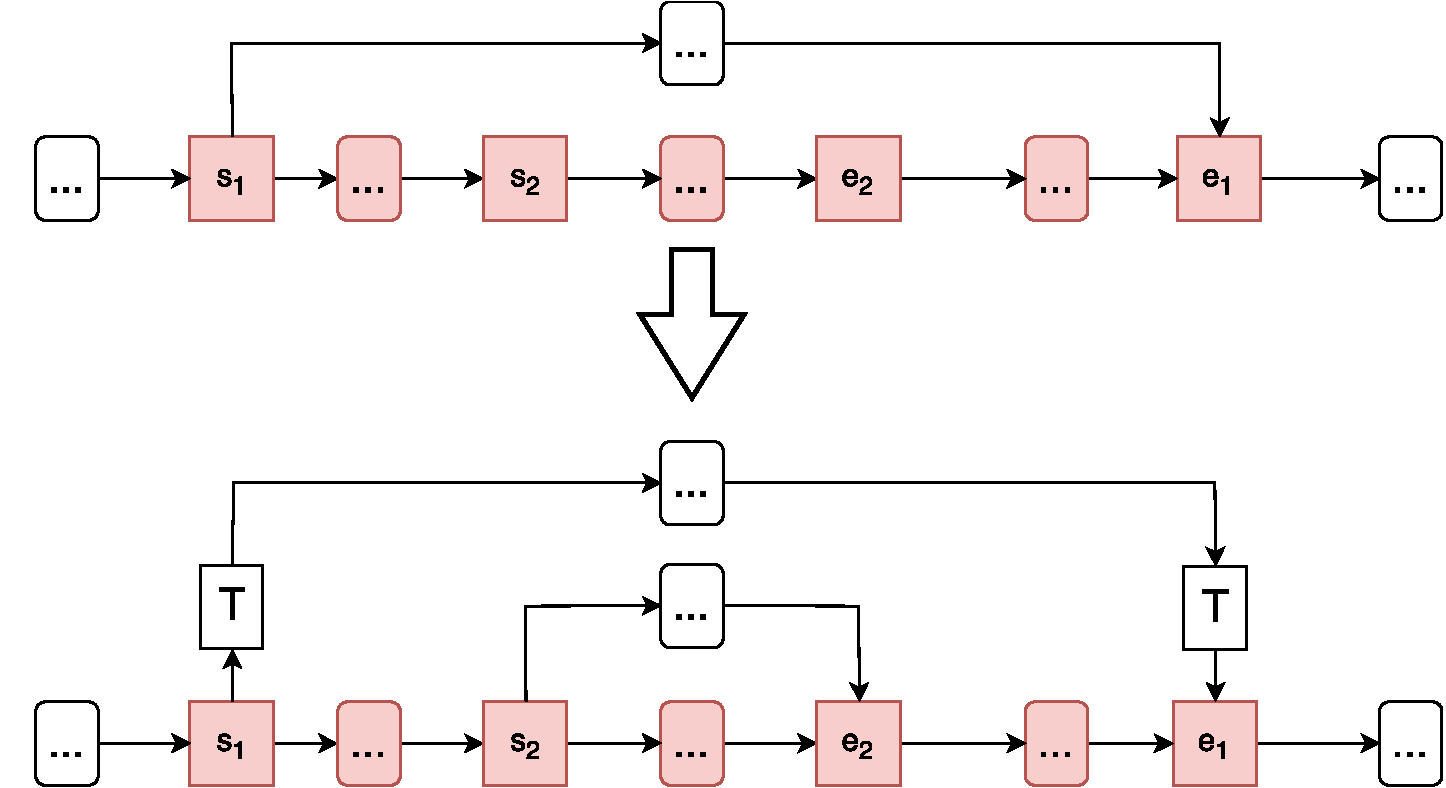
\includegraphics[width=\textwidth]{conflict3.pdf}
\caption{How push underneath handles the case, where we insert a new line that is covered entirely by an old line}
\label{fig:pushunderneath1}
\end{figure}

In the case where the new line covers the old, we handle intersection as in \cref{fig:pushunderneah2}. As we push up the new line we need to push up the old. However, we need not use transport modules to reconnect the old line, instead it can be reached by flowing vertically through the new line.

Again the cases where there is a partial intersection between old and new line is easy to imagine. If the moving up of an old line creates a new intersection, we just move up the line that was already set in place. This is done until no more intersections occur. When this has been done, some old lines may have been disconnected from their main line. We handle this by allowing items to reach them by moving vertically through existing modules and appending transport modules when needed.  

As can be seen, push underneath functions in a manner opposite to push around. We decide to use it when handling intersections that occur as a result of a parallel transformation. We want our parallel lines to be close to the line, which it sprouted from, otherwise we may not reap the benefits of adding extra modules. This is not needed as much, when doing anti-serialization, which is why we use push around for that instead.

  

\begin{figure}[h]
\centering
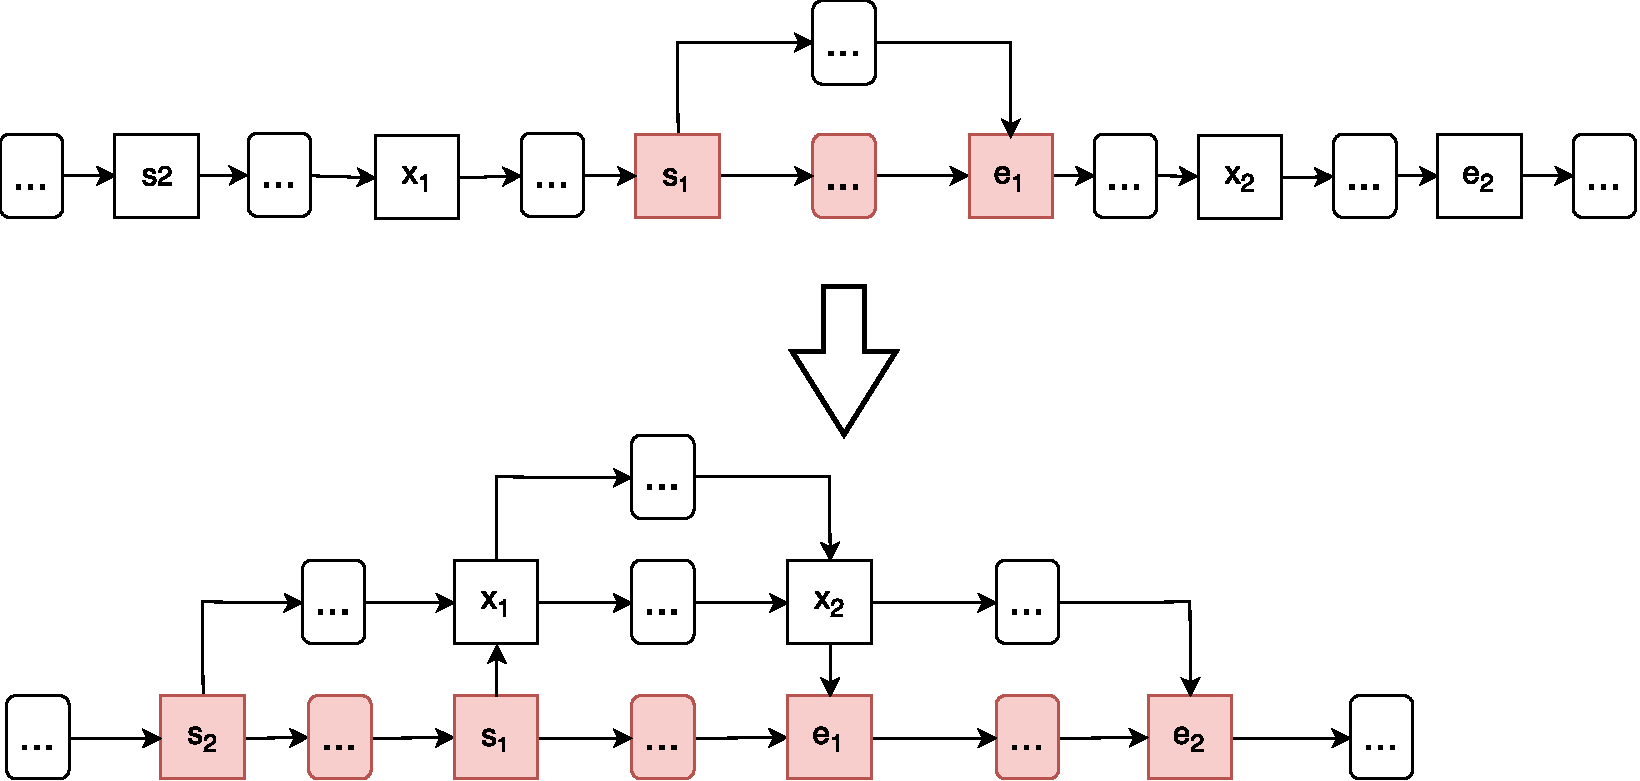
\includegraphics[width=\textwidth]{conflict4.pdf}
\caption{How push underneath handles the case, where we insert a new line that  entirely covers an an old line}
\label{fig:pushunderneath2}
\end{figure}

